\chapter{FLLOAT}\label{ch:flloat}
In this chapter, we describe \href{https://github.com/MarcoFavorito/flloat.git}{FLLOAT} (From \LLf tO AutomaTa), a software project written in Python. It is a porting of the \href{https://github.com/RiccardoDeMasellis/FLLOAT}{homonym software project} written in Java. It is the implementation of many of the topics described in Chapter \ref{ch:logic}. 
%We'll see the main features, the package structure, and some code examples.

\section{Introduction}
\paragraph{Main features:} FLLOAT is a Python library that provides support for:
\begin{itemize}
	
	\item Syntax, semantics and parsing of the following logic formalisms:
	\begin{itemize}
		\item Propositional Logic;
		\item Linear Temporal Logic on Finite Traces \LTLf
		\item Linear Dynamic Logic on Finite Traces \LDLf;
	\end{itemize}
	\item Conversion from \LLf formula to \NFA, \DFA and \DFA On-The-Fly
	
\end{itemize}

\paragraph{Dependencies:} FLLOAT requires Python>=3.5 and depends on the following packages:
\begin{itemize}
	\item \href{http://www.dabeaz.com/ply/ply.html}{PLY}, a pure-Python implementation of the popular compiler construction tools \href{http://dinosaur.compilertools.net/}{Lex and Yacc}. It has been used for the parsing of \PL and \LLf formulas;
	\item \href{https://github.com/MarcoFavorito/pythomata}{Pythomata}, a Python package which provides support for \NFA, \DFA, determinization and minimization algorithms and reasoning on \DFAs. It has been used for deal with $\automaton_\varphi$, the equivalent automaton of a \LLf formula.
\end{itemize}

\paragraph{Installation:} You can find the package on \href{https://pypi.org/project/flloat/}{PyPI}, hence you can install it with:
\begin{lstlisting}[language=bash]
pip install flloat
\end{lstlisting}
Please go \href{https://github.com/MarcoFavorito/flloat#install}{here} for further details.

The software is open source and is released under \href{https://github.com/MarcoFavorito/flloat/blob/master/LICENSE}{MIT license}.

\section{Package structure}
The package is structured as follows:
\begin{itemize}
	\item \texttt{flloat.py}: the main module, it contains the implementation of the translation from \LLf formulas to automata. The functions implemented here are called from methods of \LLf formulas.
	\item \texttt{base/}: contains the abstract definitions used in other modules. The main modules are:
	\begin{itemize}
		\item \texttt{Symbol.py} and \texttt{Symbols.py}, where have been defined the class \texttt{Symbol} to represent the atomic propositional symbols and the operator symbols;
		\item \texttt{Alphabet.py}, which is an abstraction for manage a set of \texttt{Symbol};
		\item \texttt{Interpretation.py}, an abstract class denoting the semantics used for truth evaluation. E.g. for \PL the corresponding interpretation is \texttt{PLInterpretation} (a set of \texttt{Symbol}), whereas for \LLf we have \texttt{FiniteTrace}, which is a list of \texttt{PLInterpretation}.
		\item \texttt{Formula.py}, the module containing the base class \texttt{Formula}. Every formula class extends \texttt{Formula}. In this module are defined also \texttt{AtomicFormula}, \texttt{Operator}, \texttt{BinaryOperator} etc., and how to build a syntax tree. 
		\item \texttt{truths.py} and \texttt{nnf.py} that provide abstract implementations for truth evaluations of formulas and negation normal form operations.
		\item other abstractions definitions that are implemented for each extending subclass.
	\end{itemize}
	\item \texttt{syntax/}: modules for each formalism (i.e. \texttt{pl.py}, \texttt{ltlf.py} and \texttt{ldlf.py}). In those modules are declared all the classes for representing formulas, implementing their truth evaluation procedure  taking into account their correlation (e.g. \texttt{And} is the negative dual of \texttt{Or}, you can define \texttt{Implies} in terms of \texttt{Not} and \texttt{Or} etc.);
	\item \texttt{semantics/}: modules providing implementations for the semantics. E.g. you can find \texttt{PLInterpretation} and \texttt{FiniteTrace} cited before;
	\item \texttt{parser/}: modules where are defined the parsers of formulas in \PL and \LLf. They depends on PLY.
\end{itemize}
In the following sections we show typical use cases, describe the used APIs and look at their implementation.

\section{Propositional Logic formulas}\label{sect:flloat-pl}

FLLOAT provides support for Propositional Logic (\PL). In the following, we will see both examples and explanation of the code.

\subsection{Specify a \PL formula}\label{sect:flloat-pl-syntax}
The easiest way to specify a propositional formula is to use a \texttt{PLParser}:

\begin{lstlisting}[language=Python, style=Python]
from flloat.parser.pl import PLParser

parser = PLParser()
\end{lstlisting}
For instance, the propositional formula $\varphi= A \lAND (\lnot B \lOR C) \lAND D$ can be represented in this way:

\begin{lstlisting}[language=Python, style=Python]
phi = parser("A & (!B | C) & D")
\end{lstlisting}
Which generate the syntax tree in Figure \ref{fig:pl-formula-example-1-syntax-tree}. The logical operators symbols $\lnot, \lAND, \lOR$ are replaced by, respectively, \texttt{!}, \texttt{\&}, \texttt{|}. In red are represented the symbols used to build the formula, for which the associated class is \texttt{Symbol}. On the other hand, in blue are shown the classes used to build the syntax tree, that represent a particular formula/operator in \PL. They are: \texttt{PLAtomic}, used to represent atomic propositions; \texttt{PLNot}, \texttt{PLAnd} and \texttt{PLOr} for the associated logic operators. All of them extends from the base class \texttt{Formula}.


\begin{figure}[h]
	\centering
	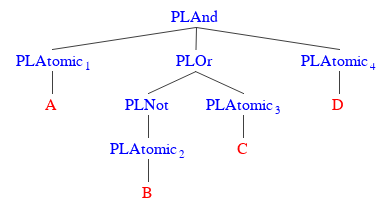
\includegraphics[width=0.5\textwidth]{images/pl-formula-example-1-syntax-tree}
	\caption{The syntax tree generated by the parsing of \texttt{"A \& (!B | C) \& D"}, In red are represented instances of the class \texttt{Symbol} , whereas in blue the instances of the formulas/operators classes used to build the syntax tree.}
	\label{fig:pl-formula-example-1-syntax-tree}
	
\end{figure}

We could construct the same syntax structure by using other APIs of FLLOAT:

\begin{lstlisting}[language=Python, style=Python, label={code:pl-syntax-example-manual}, caption={A "manually" constructed \PL formula.}]
from flloat.base.Symbol import Symbol
from flloat.syntax.pl import PLAtomic, PLAnd, PLOr, PLNot

A, B = Symbol("A"), Symbol("B")
C, D = Symbol("C"), Symbol("D")

atomic_A = PLAtomic(A)
atomic_B = PLAtomic(B)
atomic_C = PLAtomic(C)
atomic_D = PLAtomic(D)

not_B = PLNot(atomic_B)
B_or_C = PLOr([not_B, atomic_C])
phi = PLAnd([atomic_A, B_or_C, atomic_D])
\end{lstlisting}

Now follow the implementation details about how the above code can run.

\subsubsection{The \texttt{Symbol} class}
\href{https://github.com/MarcoFavorito/flloat/blob/0.1.4/flloat/base/Symbol.py#L6-L14}{\texttt{Symbol}} is one of the base classes, declared in \href{https://github.com/MarcoFavorito/flloat/blob/0.1.4/flloat/base/Symbol.py}{Symbol.py}, whose code is reported in Listing \ref{code:Symbol}.

\begin{lstlisting}[language=Python, style=Python, escapechar = £, label={code:Symbol}, caption={The \texttt{Symbol} class.}]
class Symbol(str, Hashable):
  def __init__(self, name:str):
    str.__init__(self)
    Hashable.__init__(self)
    self.name = name
    
  def _members(self):
    return self.name

\end{lstlisting}

The class \texttt{Symbol} can be thought as a wrapper for the type \texttt{str}. Additionally, it inherits some useful properties from the class \href{https://github.com/MarcoFavorito/flloat/blob/0.1.4/flloat/base/hashable.py#L1-L31}{\texttt{Hashable}}, implemented for performance purposes, which is reported in Listing \ref{code:Hashable}:

\begin{lstlisting}[language=Python, style=Python, escapechar = £, label={code:Hashable}, caption={The \texttt{Hashable} class.}]
from abc import ABC, abstractmethod
from copy import copy

class Hashable(ABC):

  def __init__(self):
    self._hash = None

  @abstractmethod
  def _members(self):
    raise NotImplementedError

  def __eq__(self, other):
    if type(other) is type(self):
      return self._members() == other._members()
    else:
      return False

  def __hash__(self):
    if self._hash is None:
      self._hash = hash(self._members())
    return self._hash

  def __getstate__(self):
    d = copy(self.__dict__)
    d.pop("_hash")
    return d

  def __setstate__(self, state):
    self.__dict__ = state
    self._hash = None
\end{lstlisting}

Its main purpose is to allow memoization of the hash value. This is useful for immutable objects since their hash value does not change during their life cycle. Furthermore, the mathematical domain of interest requires hash-based data structure such as sets and dictionaries, so it is a good idea to compute the hash only once and retrieve the precomputed value when needed. The \texttt{Hashable} class is inherited from many other classes since the immutable property is satisfied by many entities. It requires that all the classes that inherit from it implement a \texttt{\_\_members} function, which returns a hashable signature of the object that identifies it uniquely. The methods \texttt{\_\_getstate\_\_} and \texttt{\_\_setstate\_\_} simply do not include the precomputed hash value, since it might have a different value among different Python processes, due to hash randomization.


\subsubsection{The \texttt{Formula} abstract class and other abstraction}
In \href{https://github.com/MarcoFavorito/flloat/blob/0.1.4/flloat/base/Formula.py}{\texttt{flloat/base/Formula.py}} there are many abstraction that allow the construction of the syntax tree. The three dots \texttt{...} represent code omissions. 

\begin{lstlisting}[language=Python, style=Python, escapechar = £, label={code:Formula.py}, caption={\texttt{flloat/base/Formula.py}} module]
from abc import abstractmethod, ABC
from typing import Sequence, Set

from flloat.base.Symbol import Symbol
from flloat.base.Symbols import Symbols
from flloat.base.hashable import Hashable


class Formula(Hashable):
  def __init__(self):
    super().__init__()
    
    ...

class AtomicFormula(Formula):
  def __init__(self, s:Symbol):
    super().__init__()
    self.s = s

  def _members(self):
    return self.s

  ...
  
class Operator(Formula):
  @property
  def operator_symbol(self) -> str:
    raise NotImplementedError
    
    ...

class UnaryOperator(Operator):
  def __init__(self, f: Formula):
    super().__init__()
    self.f = f.simplify()

  def _members(self):
    return (self.operator_symbol, self.f)

  ...

class BinaryOperator(Operator):
  def __init__(self, formulas:OperatorChilds):
    super().__init__()
    assert len(formulas) >= 2
    self.formulas = tuple(formulas)
    self.formulas = self._popup()
	
  ...
  
  def _members(self):
    return (self.operator_symbol, self.formulas)

  def _popup(self):
    """recursively find the same binary operator among 
    child formulas and pop up them at the same level"""
    res = ()
    for child in self.formulas:
      if type(child) == type(self):
        superchilds = child._popup()
        res += superchilds
      else:
        res += (child, )
    return tuple(res)

class CommutativeBinaryOperator(BinaryOperator):
  def __init__(self, formulas:OperatorChilds):
    # Assuming idempotence: e.g. A & A === A
    super().__init__(formulas)
    # order does not matter -> set operation
    # remove duplicates -> set operation
    self.formulas_set = frozenset(self.formulas)
    # unique representation -> sorting
    self.members = tuple(
      sorted(self.formulas_set, key=lambda x: hash(x))
    )
      
   ...

\end{lstlisting}

The class \texttt{Formula} is "the mother" of all the formulas. \texttt{AtomicFormula} represents a formula without any child in the syntax tree; it holds a \texttt{Symbol} object. \texttt{Operator} is an abstract class that represents a logical operator over formulas. It can be a \texttt{UnaryOperator} (e.g. the \emph{not} $\lnot$), a \texttt{BinaryOperator} (e.g. the \emph{implies} $\Rightarrow$) and a \texttt{CommutativeBinaryOperator}, which is a binary operator that satisfies the commutative property (e.g. the \emph{and} $\lAND$ and the \emph{or} $\lOR$). Every \texttt{Operator} has to have an operator symbol used for the conversion into strings. 

When constructing a \texttt{BinaryOperator} instance, the list of subformulas is analyzed by looking for a subformula of the same type of the instance. This is a way to avoid multiple representations of the same syntax tree. For build a \texttt{BinaryOperator} formula, we need a \emph{list} of subformulas, whereas for a \texttt{CommutativeBinaryOperator} we hold subformulas as a \emph{set}, because order does not matter. However, for the latter case, in order to have a unique representation, we hold also a list of subformulas sorted by their hash.

We remark that,despite the name, \texttt{BinaryOperator} constructor take as input a \emph{list} of formulas and not a \emph{pair} of formulas. The reason, as stated before, is to reduce the depth of the syntax tree when the same binary operator is applied in chain many times.

Figure \ref{fig:formula-diagram} depicts a schema to represent the relations between the just described abstractions.

\begin{figure}
	\centering
	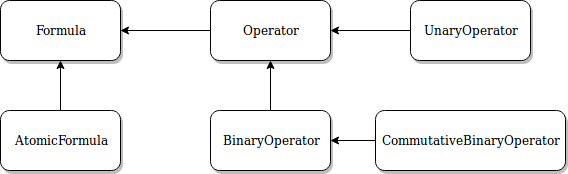
\includegraphics[width=0.9\textwidth]{images/formula-diagram}
	\caption{An inheritance schema for the classes in \href{https://github.com/MarcoFavorito/flloat/blob/0.1.4/flloat/base/Formula.py}{\texttt{flloat/base/Formula.py}}. Arrows stand for "extends".}
	\label{fig:formula-diagram}
\end{figure}

\subsubsection{\texttt{PLFormula}s: \texttt{PLAtomic}, \texttt{PLNot}, \texttt{PLAnd}, \texttt{PLOr} classes}
The \texttt{PLAtomic}, \texttt{PLNot}, \texttt{PLAnd}, \texttt{PLOr} classes, as well as other \PL classes for syntax support, are all declared in \href{https://github.com/MarcoFavorito/flloat/blob/0.1.4/flloat/syntax/pl.py}{\texttt{flloat/syntax/pl.py}} (Listing \ref{code:syntax-pl.py}). 

\begin{lstlisting}[language=Python, style=Python, escapechar = £, label={code:syntax-pl.py}, caption={The \href{https://github.com/MarcoFavorito/flloat/blob/0.1.4/flloat/syntax/pl.py}{\texttt{flloat/syntax/pl.py}} module}]
class PLTruth(Truth):
  @abstractmethod
  def truth(self, i: PLInterpretation, *args):
    raise NotImplementedError

class PLFormula(Formula, PLTruth, NNF):
  def __init__(self):
    Formula.__init__(self)

  def all_models(self, alphabet: _Alphabet):
  """Find all the possible interpretations 
  given a set of symbols"""
    ...

  def minimal_models(self, alphabet: _Alphabet):
  """Find models of minimum size"""
    ...

class PLBinaryOperator(BinaryOperator, PLFormula):
  ...

class PLCommBinaryOperator(DualCommutativeOperatorNNF,
  PLFormula):
  ...

class PLAtomic(AtomicFormula, PLFormula):

  def truth(self, i:PLInterpretation, *args)£\label{code:pl-syntax-truth-PLAtomic}£:
    return self.s in i

  def _to_nnf(self):
    return self

 def negate(self):
    return PLNot(self)

class PLTrue(PLAtomic):
  def __init__(self):
    PLAtomic.__init__(self, Symbol(Symbols.TRUE.value))

  def truth(self, *args)£\label{code:pl-syntax-truth-PLTrue}£:
    return True

  def negate(self):
    return PLFalse()


class PLFalse(PLAtomic):
  def __init__(self):
    PLAtomic.__init__(self, Symbol(Symbols.FALSE.value))

  def truth(self, *args)£\label{code:pl-syntax-truth-PLFalse}£:
    return False

  def negate(self):
    return PLTrue()

class PLNot(NotTruth, PLFormula, NotNNF):
  pass

class PLOr(PLCommBinaryOperator, OrTruth):
  pass

class PLAnd(PLCommBinaryOperator, AndTruth):
  pass

class PLImplies(PLBinaryOperator, ImpliesConvertible):
  And = PLAnd
  Or = PLOr
  Not = PLNot

class PLEquivalence(PLCommBinaryOperator, 
  EquivalenceConvertible):
  And = PLAnd
  Or = PLOr
  Not = PLNot

PLOr.Dual = PLAnd
PLAnd.Dual = PLOr

\end{lstlisting}
Every propositional formula extends from \texttt{PLFormula}. It implements the methods \texttt{all\_models} that, given an alphabet, returns all the propositional interpretations that satisfy the formula. \texttt{minimal\_models} returns only the minimal ones. \texttt{PLBinaryOperator} and \texttt{PLCommBinaryOperator} are conceptually the same of \texttt{BinaryOperator} and \texttt{CommutativeBinaryOperator} described before. 

Other classes define the possible \PL formulas: \texttt{PLAtomic} is an \texttt{AtomicFormula}, hence its instances just hold a \texttt{Symbol} object; \texttt{PLTrue} and \texttt{PLFalse} are \texttt{PLAtomic} formulas with a fixed symbol that represent, respectively, propositional $\true$ and propositional $\false$; \texttt{PLNot}, \texttt{PLAnd}, \texttt{PLOr} has been already described; \texttt{PLImplies} and \texttt{PLEquivalence} correspond to $\Rightarrow$ and $\Leftrightarrow$ logic operator, respectively.

It is interesting to observe that the implementation of some features such as syntax, semantics and conversion to Negation Normal Form (NNF) is inherited from other classes/interfaces, such as \texttt{Truth} and \texttt{NNF}. The implementation is made generically, i.e. by not assuming that we are talking about \PL formulas. Indeed, the implementation of the same formulas (and, or, not etc.) is used for \PL and \LLf. We will discuss them in the next sections.

\subsection{Parsing of \PL formulas}\label{sect:flloat-pl-parsing}
Here we describe how the parsing of a string, representing a \PL formula. to an instance of \texttt{PLFormula}, works. The implementation of the \PL formula parsing is provided by the class \texttt{PLParser}, declared in the module \href{https://github.com/MarcoFavorito/flloat/blob/0.1.4/flloat/parser/pl.py}{flloat/parser/pl.py}.
In Listing \ref{code:pl-parsing-example} is shown an example of use of this feature. The formula to be parsed is $A \lAND (\lnot B \lOR C) \lAND D$. The associated string that \texttt{PLParser} is able to understand is \texttt{A \& (!B | C) \& D}.

\begin{lstlisting}[language=Python, style=Python, escapechar = £, label={code:pl-parsing-example}, caption={How to parse a \PL formula: \texttt{PLParser}}]
from flloat.parser.pl import PLParser
parser = PLParser()
phi = parser("A & (!B | C) & D")
\end{lstlisting}

In Listing \ref{code:PLLexer-PLParser} are shown the implementation of \texttt{PLParser} and the associated lexer, \texttt{PLLexer}. They extends a more general definition of \texttt{Parser} and \texttt{Lexer}, implemented in the module \href{https://github.com/MarcoFavorito/flloat/blob/0.1.4/flloat/base/parsing.py}{flloat/base/parsing.py}.
\begin{lstlisting}[language=Python, style=Python, escapechar = £, label={code:PLLexer-PLParser}, caption={\texttt{PLLexer} and \texttt{PLParser}}]
class PLLexer(Lexer):

  def __init__(self):
    super().__init__()

  reserved = {
      Symbols.TRUE.value  : 'TRUE',
      Symbols.FALSE.value : 'FALSE',
  }

  # List of token names.   This is always required
  tokens = (
  'ATOM',
  'NOT',
  'AND',
  'OR',
  'IMPLIES',
  'EQUIVALENCE',
  'LPAREN',
  'RPAREN'
  ) + tuple(reserved.values())

  # Regular expression rules for simple tokens
  t_NOT          = sym2regexp(Symbols.NOT)
  t_AND          = sym2regexp(Symbols.AND)
  t_OR           = sym2regexp(Symbols.OR)
  t_IMPLIES      = sym2regexp(Symbols.IMPLIES)
  t_EQUIVALENCE  = sym2regexp(Symbols.EQUIVALENCE)
  t_LPAREN       = sym2regexp(Symbols.ROUND_BRACKET_LEFT)
  t_RPAREN       = sym2regexp(Symbols.ROUND_BRACKET_RIGHT)



  def t_ATOM(self, t):£\label{code:pl-parser-atom-token-regex}£
    r'[a-zA-Z_][a-zA-Z_0-9]*'
    # Check for reserved words
    t.type = PLLexer.reserved.get(t.value, 'ATOM')  
    return t


# Yacc 
class PLParser(Parser):

  def __init__(self):
    lexer = PLLexer()
    precedence = (
      ('left', 'EQUIVALENCE'),
      ('right', 'IMPLIES'),
      ('left', 'OR'),
      ('left', 'AND'),
      ('right', 'NOT'),
      )
    super().__init__("pl", lexer.tokens, lexer, precedence)

  def p_formula_atom(self, p):£\label{code:pl-parsing-atom}£
  """formula : ATOM
             | TRUE
             | FALSE"""
    if p[1]==Symbols.TRUE.value:
     p[0] = PLTrue()
    elif p[1]==Symbols.FALSE.value:
      p[0] = PLFalse()
    else:
      p[0] = PLAtomic(Symbol(p[1]))

  def p_formula_not(self, p):
  'formula : NOT formula'
    p[0] = PLNot(p[2])

  def p_formula_or(self, p):
  'formula : formula OR formula'
    p[0] = PLOr([p[1], p[3]])

  def p_formula_and(self, p):
  'formula : formula AND formula'
    p[0] = PLAnd([p[1], p[3]])

  def p_formula_implies(self, p):
  'formula : formula IMPLIES formula'
    p[0] = PLImplies([p[1], p[3]])

  def p_formula_equivalence(self, p):
  'formula : formula EQUIVALENCE formula'
    p[0] = PLEquivalence([p[1], p[3]])

  def p_formula_expression(self, p):
  'formula : LPAREN formula RPAREN'
    p[0] = p[2]
\end{lstlisting}
This feature depends from PLY, which provides utilities for both tokenization and parsing of a string. We do not go into details about how PLY works. 

For the lexer part, we defied the available tokens for the parsing phase, as well as reserved words/symbols/regular expression for each of them (e.g. look at the regex for the \texttt{ATOM} token at line \ref{code:pl-parser-atom-token-regex}). The symbols used for the operators are defined in the module \href{https://github.com/MarcoFavorito/flloat/blob/0.1.4/flloat/base/Symbols.py}{flloat/base/Symbols.py}.

For the parsing part, we defined how to construct a syntax tree from the list of tokens. For each type of formula, we defined inductively a set of rules that, when activated, create the proper \texttt{PLFormula} object.

For example, consider line \ref{code:pl-parsing-atom}, where has been defined the rule to generate the atomic formulas. Depending on the type of token that activated the rule, we generate a \texttt{PLTrue}, \texttt{PLFalse} or a \texttt{PLAtomic} formula with the symbol provided by the tokenizer. Analogous considerations are made for other types of rules and formulas.
Eventually, when there is no rule to apply, the entire syntax tree has been built. The object that we built "manually" (see Listing \ref{code:pl-syntax-example-manual}) now is built automatically by the parser.

This pattern is the same used for \LLf parsers.

\subsection{\PL formulas evaluation}\label{sect:flloat-pl-semantics}
In this section, we see how to compute the truth value of a  \texttt{PLFormula}, given a propositional interpretation. 
We represent the propositional interpretation with the class \href{https://github.com/MarcoFavorito/flloat/blob/0.1.4/flloat/semantics/pl.py#L8-L28}{\texttt{PLInterpretation}}, that is trivially a set of \texttt{Symbol}s (the ones that we consider true).


\begin{lstlisting}[language=Python, style=Python, escapechar = £, label={code:pl-semantics-example}, caption={An example for \PL formula truth evaluation}]
from flloat.parser.pl import PLParser
parser = PLParser()
phi = parser("A & (!B | C) & D")

from flloat.semantics.pl import PLInterpretation

A_true = PLInterpretation.fromStrings(["A"])
print(phi.truth(A_true)) #prints False
ACD_true = PLInterpretation.fromStrings(["A", "C", "D"])
print(phi.truth(ACD_true)) #prints True
\end{lstlisting}

You can notice that we can easily define a \texttt{PLInterpretation} by using the static method \texttt{fromStrings} and providing a collection of strings corresponding to the propositions that we want to make $true$. The evaluation is made by the method \texttt{truth}, that is implemented by every \texttt{PLFormula}. As stated in Section \ref{sect:flloat-pl-syntax}, the actual implementation of the (trivial) procedures to evaluate the truths of logic operators are defined in \href{https://github.com/MarcoFavorito/flloat/blob/0.1.4/flloat/base/truths.py}{flloat/base/truths.py}, that are inherited by the different \texttt{PLFormula}s. The truth evaluation of atomic formulas such as \texttt{PLAtomic}, \texttt{PLTrue} and \texttt{PLFalse} are, respectively, in lines \ref{code:pl-syntax-truth-PLAtomic}, \ref{code:pl-syntax-truth-PLTrue} and \ref{code:pl-syntax-truth-PLFalse} of Listing \ref{code:syntax-pl.py}.

In Figure \ref{fig:formula-diagram-pl-truths} is depicted the schema representing the relations between the classes used for logic formulas discussed until now. It is worth to notice the separation between the implementation of the syntax and the one of the semantics, from where the propositional formula classes inherit their functionalities. This organization is replicated in both \LTLf and \LDLf implementations.

\begin{sidewaysfigure}[h]
	\centering
	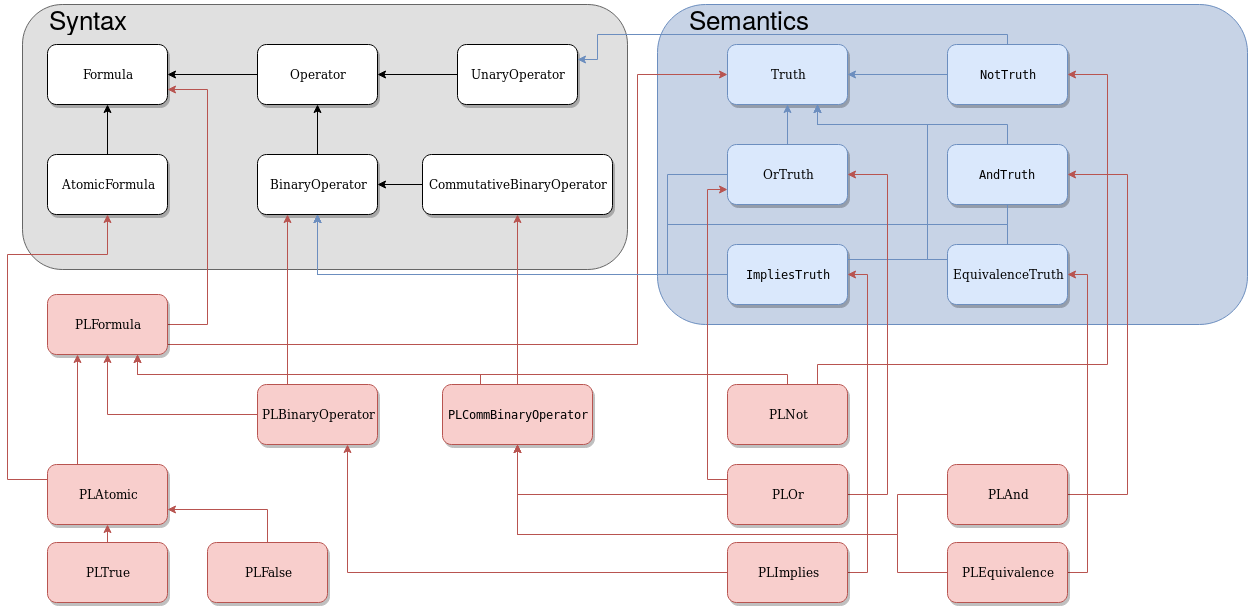
\includegraphics[width=\textwidth]{images/pl-formula-diagram-truth}
	\caption{A schema representing the relations between the FLLOAT classes, that extends the one in Figure \ref{fig:formula-diagram}. The arrows mean "extends". In white the classes that implement how the syntax tree is built. In light blue the classes that implement the truth evaluation of operators. In red the classes that represent \PL formulas. \PL classes inherits from both syntax classes and semantics classes without implementing again both syntax and semantics functionalities.}
	\label{fig:formula-diagram-pl-truths}
\end{sidewaysfigure}
\clearpage

%formula = "<true*; A & B>tt"
%# returns a LDLfFormula
%parsed_formula = parser(formula)        
%
%# prints "<((true)* ; (A & B))>(tt)"
%print(parsed_formula)                   
%# prints {A, B}
%print(parsed_formula.find_labels())


\section{\LTLf formulas}\label{sect:flloat-ltlf}
As stated before, the software architecture to support \LLf formulas is pretty the same of the one presented in Section \ref{sect:flloat-pl}. The core syntax functionalities (i.e. how to build the syntax tree of a \LLf formula) are inherited from the classes defined in \href{https://github.com/MarcoFavorito/flloat/blob/0.1.4/flloat/base/Formula.py}{\texttt{flloat/base/Formula.py}}, as described in Section \ref{sect:flloat-pl-syntax}. The semantics functionalities for propositional logic operator (e.g. And, Or, Not) are inherited from \texttt{Truth}s classes declared in \href{https://github.com/MarcoFavorito/flloat/blob/0.1.4/flloat/base/truths.py}{flloat/base/truths.py} (see Section \ref{sect:flloat-pl-semantics}). Other ad-hoc data structures and classes are defined in order to support \LLf formulas.

In this section, we describe the \LTLf part analogously to what we did in Section \ref{sect:flloat-pl} for \PL. In the next section, we do the same for \LDLf.

\subsection{Specify \LTLf formulas}\label{sect:flloat-ltlf-syntax}
In this section, we will see how to build \LTLf formulas.

In Listing \ref{code:ltlf-syntax-example} is shown the construction of the main \LTLf formulas.

\begin{lstlisting}[language=Python, style=Python, escapechar = £, label={code:ltlf-syntax-example}, caption={Examples of \LTLf formulas}]
from flloat.base.Symbol import Symbol
from flloat.syntax.ltlf import LTLfAtomic, LTLfAnd,\
LTLfOr, LTLfNot, LTLfImplies, LTLfEquivalence,\
LTLfNext, LTLfWeakNext, LTLfUntil, LTLfRelease, \
LTLfAlways, LTLfEventually
A_sym, B_sym = Symbol("A"), Symbol("B")
A = LTLfAtomic(A_sym)
B = LTLfAtomic(B_sym)

# classic logic operators
A_and_B = LTLfAnd([A, B])
A_or_B = LTLfOr([A, B])
not_A = LTLfNot(A)
A_implies_B = LTLfImplies([A, B])
A_equivalence_B = LTLfEquivalence([A, B])

#temporal operators
next_A = LTLfNext(A)
wnext_A = LTLfWeakNext(A)
A_until_B = LTLfUntil([A, B])
A_release_B = LTLfRelease([A, B])
always_A = LTLfAlways(A)
eventually_A = LTLfEventually(A)
\end{lstlisting}
All the classes for construct \LTLf formulas are declared in \href{https://github.com/MarcoFavorito/flloat/blob/0.1.4/flloat/syntax/ltlf.py}{flloat/syntax/ltlf.py}.
The formula \texttt{LTLfAtomic} and the operators \texttt{LTLfAnd}, \texttt{LTLfOr}, \texttt{LTLfNot}, \texttt{LTLfImplies} and \texttt{LTLfEquivalence} are conceptually the same of the \PL formulas described in Section \ref{sect:flloat-pl-syntax}. They extends \texttt{LTLfFormula} instead of \texttt{PLFormula} and inherits the syntax functionalities from the base classes in \texttt{flloat/base/Formula.py}.

The novelty is about the temporal formulas \texttt{LTLfNext}, \texttt{LTLfWeakNext}, \texttt{LTLfUntil}, \texttt{LTLfRelease}, \texttt{LTLfAlways} and \texttt{LTLfEventually}, each of them extending \texttt{LTLfTemporalFormula}, which in turn extends \texttt{LTLfFormula}. They inherit the syntax functionalities from \texttt{UnaryOperator} and \texttt{BinaryOperator}, in a straightforward way.

Observe that the operators \texttt{LTLfWeakNext}, \texttt{LTLfRelease}, \texttt{LTLfAlways} and \texttt{LTLfEventually} are \emph{abbreviations}, in the sense that they can be rewritten by only using combinations of \texttt{LTLfNot}, \texttt{LTLfNext} and \texttt{LTLfUntil}. In order to reuse the code as much as possible, the relevant methods of these operators (such as \texttt{truth} or \texttt{to\_nnf}, which put the formula in NNF) actually first \emph{convert} the formula to an equivalent one by using only $\lnot, \Next, \lUntil$, and then call the method on the newly created formula.

In order to do that, these classes extends the \texttt{BaseConvertibleFormula} declared in \href{https://github.com/MarcoFavorito/flloat/blob/0.1.4/flloat/base/convertible.py}{flloat/base/convertible.py} (Listing \ref{code:base-convertible-formula}). This concept is used also in the implementation of support for \LDLf formulas.

\begin{lstlisting}[language=Python, style=Python, escapechar = £, label={code:base-convertible-formula}, caption={The \texttt{BaseConvertibleFormula} abstraction, in \href{https://github.com/MarcoFavorito/flloat/blob/0.1.4/flloat/base/convertible.py}{flloat/base/convertible.py}.}]
...

class ConvertibleFormula(Formula):
@abstractmethod
def _convert(self):
raise NotImplementedError

class BaseConvertibleFormula(ConvertibleFormula, Truth, NNF):
def truth(self, *args):
return self._convert().truth(*args)

def _to_nnf(self):
return self._convert().to_nnf()

def negate(self):
return self._convert().negate()

...
\end{lstlisting}

Indeed, by continuing from  Listing \ref{code:ltlf-syntax-example}:
\begin{lstlisting}[language=Python, style=Python]
print(wnext_A._convert())      #prints '!(X(!(A)))'
print(A_release_B._convert())  #prints '!((!(A) U !(B)))'
print(eventually_A._convert()) #prints '(true U A)'
print(always_A._convert())     #prints '!((true U !(A)))'
\end{lstlisting}

\subsubsection{\texttt{LTLfFormula}: the base abstraction for \LTLf formulas}

In Listing \ref{code:ltlf-syntax-LTLfFormula} is shown the implementation of \texttt{LTLfFormula}, which is extended by every \LTLf formula class. It extends the following classes (skipping the class \texttt{Formula}):
\begin{itemize}
\item \texttt{LTLfTruth} (line \ref{code:ltlf-syntax-LTLfTruth}) which defines the method \texttt{truth} that takes in input a \texttt{FiniteTrace} (see Section \ref{ltlf-semantics} and Section \ref{sect:flloat-ltlf-semantics}) and a position from which evaluate the trace (by default 0, i.e. from the beginning).
\item \texttt{NNF}, a class which defines the abstract method \texttt{to\_nnf} that returns the same formula but in Negation Normal Form (NNF);
\item \texttt{Delta}, a class which defines the abstract method \texttt{\_delta}, (line \ref{code:ltlf-_delta-method}) called from \texttt{delta} (line \ref{code:ltlf-delta-method}), that implements the delta function described in Section \ref{ltlf-delta-section}.
\end{itemize}

Every subclass implements those methods properly, by taking into account the definitions provided in Section \ref{ltlf-semantics} and Section \ref{ltlf-delta-section}.

\begin{lstlisting}[language=Python, style=Python,  escapechar = £, label={code:ltlf-syntax-LTLfFormula}, caption={The \texttt{LTLfFormula} abstraction (\href{https://github.com/MarcoFavorito/flloat/blob/0.1.4/flloat/syntax/ltlf.py}{flloat/syntax/ltlf.py)}}]
class LTLfTruth(Truth):£\label{code:ltlf-syntax-LTLfTruth}£
  @abstractmethod
  def truth(self, i: FiniteTrace, pos: int = 0):
    raise NotImplementedError


class LTLfFormula(Formula, LTLfTruth, NNF, Delta):

  @lru_cache(maxsize=MAX_CACHE_SIZE)£\label{code:ltlf-delta-method}£
  def delta(self, i: PLInterpretation, epsilon=False):£\label{code:ltlf-delta-method}£
    f = self.to_nnf()
    d = f._delta(i, epsilon)
    if epsilon:
      # By definition, if epsilon=True, then 
      #the result must be either PLTrue or PLFalse
      # Now, the output is a Propositional Formula
      # with only PLTrue or PLFalse as atomics
      # Hence, we just evaluate the formula with a dummy PLInterpretation
      d = PLTrue() if d.truth(None) else PLFalse()
    return d

  @abstractmethod
  def _delta(self, i: PLInterpretation, epsilon=False):£\label{code:ltlf-_delta-method}£
  """apply delta function, assuming that 'self' is a 
  LTLf formula in Negative Normal Form"""
    raise NotImplementedError

  @abstractmethod
  def to_LDLf(self):£\label{code:ltlf-to-ldlf-method}£
    raise NotImplementedError

  def to_automaton(self, labels:Set[Symbol]=None, on_the_fly=False,
   determinize=False, minimize=True):£\label{code:ltlf-to-automaton-method}£
    if labels is None:
      labels = self.find_labels()
    if on_the_fly:
      return DFAOTF(self)
    elif determinize:
      return to_automaton(self, labels, minimize)
    else:
      return to_automaton_(self, labels)
\end{lstlisting}
For the \texttt{delta} function it has been used a LRU caching mechanism, provided from the Python Standard Library \href{https://docs.python.org/3/library/functools.html}{\texttt{functools}}. This is needed in order to speed-up the expensive and repeated computation of the function \texttt{delta}.

At line \ref{code:ltlf-to-ldlf-method} is defined the abstract method \texttt{to\_LDLf}, which transform the current \LTLf formula instance into an \LDLf equivalent formula (by leveraging the equivalences shown in Section \ref{sect:ldlf-semantics}). Every specific \LTLf formula class implements the procedure to transform itself into an equivalent \LDLf formula. In practice, the root formula of the \LTLf syntax tree computes the result by transforming each child into a \LDLf formula, in such a way that the entire syntax tree is properly rewritten.

At line \ref{code:ltlf-to-automaton-method} it is defined the method \texttt{to\_automaton} which transform the \LTLf formula into an equivalent automaton. We discuss it in later sections.
\subsection{Parsing of \LTLf formulas}\label{sect:flloat-ltlf-parsing}
In this part we show how to use the \LTLf parsing feature, analogously to what we did in Section \ref{sect:flloat-pl-parsing}.

In Listing \ref{code:ltlf-parsing-example} is shown an equivalent approach to build \LTLf formulas, as we did in Listing \ref{code:ltlf-syntax-example}.
\begin{lstlisting}[language=Python, style=Python, escapechar = £, label={code:ltlf-parsing-example}, caption={Parsing of \LTLf formulas}]
from flloat.parser.ltlf import LTLfParser

parser = LTLfParser()

# classic logic operators
A_and_B = parser("A & B")
A_or_B = parser("A | B")
not_A = parser("!A")
A_implies_B = parser("A -> B")
A_equivalence_B = parser("A <-> B")

#temporal operators
next_A = parser("X A")
wnext_A = parser("WX A")
A_until_B = parser("A U B")
A_release_B = parser("A R B")
always_A = parser("G A")
eventually_A = parser("F A")
\end{lstlisting}
The syntax of classic logic operators is the same of the \texttt{PLParser} presented in Section \ref{sect:flloat-pl-parsing}. The implementation of \texttt{LTLfParser} can be found in \href{https://github.com/MarcoFavorito/flloat/blob/0.1.4/flloat/parser/ltlf.py}{flloat/parser/ltlf.py}. It has been implemented in the same fashion of \texttt{PLParser}, but with more reserved symbols (\texttt{X}, \texttt{WX}, \texttt{U}, \texttt{R}, \texttt{G}, and \texttt{F} for represent, repsectively, the \LTLf operators $\Next, \Wnext, \lUntil, \Release, \Box, \Diamond$) and their associated parsing rules. Combinations and arbitrary nesting of those operators with "\texttt{(}" and "\texttt{)}" are allowed.

Notice how rules defined from line \ref{code:ltlf-parser-rules} reflects the ones defined in Section \ref{ltlf-syntax}.


\begin{lstlisting}[language=Python, style=Python, escapechar = £, label={code:ltlf-parser}, caption={An extract from \href{https://github.com/MarcoFavorito/flloat/blob/0.1.4/flloat/parser/ltlf.py}{flloat/parser/ltlf.py}.}]
class LTLfParser(Parser):

...

  def p_formula(self, p):
      """formula : formula EQUIVALENCE formula £\label{code:ltlf-parser-rules}£
                  | formula IMPLIES formula
                  | formula OR formula
                  | formula AND formula
                  | formula UNTIL formula
                  | formula RELEASE formula
                  | EVENTUALLY formula
                  | ALWAYS formula
                  | NEXT formula
                  | WEAK_NEXT formula
                  | NOT formula
                  | TRUE
                  | FALSE
                  | ATOM"""
      if len(p) == 2:
        if p[1] == Symbols.TRUE.value:
          p[0] = LTLfTrue()
        elif p[1] == Symbols.FALSE.value:
          p[0] = LTLfFalse()
        else:
          p[0] = LTLfAtomic(Symbol(p[1]))
      elif len(p) == 3:
        if p[1] == Symbols.NEXT.value:
          p[0] = LTLfNext(p[2])
        elif p[1] == Symbols.WEAK_NEXT.value:
          p[0] = LTLfWeakNext(p[2])
        elif p[1] == Symbols.EVENTUALLY.value:
          p[0] = LTLfEventually(p[2])
        elif p[1] == Symbols.ALWAYS.value:
          p[0] = LTLfAlways(p[2])
        elif p[1] == Symbols.NOT.value:
          p[0] = LTLfNot(p[2])
      elif len(p) == 4:
        l, o, r = p[1:]
        if o == Symbols.EQUIVALENCE.value:
          p[0] = LTLfEquivalence([l, r])
        elif o == Symbols.IMPLIES.value:
          p[0] = LTLfImplies([l, r])
        elif o == Symbols.OR.value:
          p[0] = LTLfOr([l, r])
        elif o == Symbols.AND.value:
          p[0] = LTLfAnd([l, r])
        elif o == Symbols.UNTIL.value:
          p[0] = LTLfUntil([l, r])
        elif o == Symbols.RELEASE.value:
          p[0] = LTLfRelease([l, r])
        else:
          raise ValueError
      else:
        raise ValueError

  def p_expr_paren(self, p):
    """formula : LPAREN formula RPAREN"""
    p[0] = p[2]
\end{lstlisting}

\subsection{\LTLf formulas evaluation}\label{sect:flloat-ltlf-semantics}
The semantics of \LTLf (as well as of \LDLf) is provided by finite traces $\trace$ over a given set of propositional symbols $\Prop$, i.e. a sequence of propositional interpretations $\PropInt\in 2^\Prop$.

FLLOAT allow to construct \texttt{FiniteTrace} instances in a easy way: providing to the static method \texttt{FiniteTrace.fromStringSets} a list of sets of strings, where each string represent a propositional symbol of interest. In Listing \ref{code:finite-trace-example} an example about how to use \texttt{FiniteTrace} is given.
\begin{lstlisting}[language=Python, style=Python,  escapechar = £, label={code:finite-trace-example}, caption={Defining a finite trace $\trace = \tup{\set{}, \set{A}, \set{A, B}}$ in FLLOAT.}]
from flloat.semantics.ldlf import FiniteTrace

t1 = FiniteTrace.fromStringSets([
  {},
  {"A"},
  {"A", "B"},
])
\end{lstlisting}

In Listing is shown how to evaluate \LTLf formulas.
\begin{lstlisting}[language=Python, style=Python,  escapechar = £, label={code:ltlf-semantics-examples}, caption={Some examples about how evaluate \LTLf formulas.}]
from flloat.parser.ltlf import LTLfParser
from flloat.semantics.ldlf import FiniteTrace

parser = LTLfParser() 

#temporal operators
next_A = parser("X A")
wnext_A = parser("WX A")
A_until_B = parser("A U B")
A_release_B = parser("A R B")
always_A = parser("G A")
eventually_A = parser("F A")

t1 = FiniteTrace.fromStringSets([
  {},
  {"A"},
  {"B"},
  {"A", "B"},
])

next_A.truth(t1) #True
next_A.truth(t1, 3) #False, at the end of the trace

wnext_A.truth(t1, 1) #False
wnext_A.truth(t1, 3) #True, at the end of the trace

A_until_B.truth(t1) #False
A_until_B.truth(t1, 3) #True

A_release_B.truth(t1) #False
A_release_B.truth(t1, 2) #True

always_A.truth(t1) #False
always_A.truth(t1, 3) #True

eventually_A.truth(t1) #True
eventually_A.truth(t1, 4) #False, beyond the end of the trace
\end{lstlisting}

For the \LTLf classic logical operators, the implementation of the semantics is exactly the same of the one used for \PL formulas (see Section \ref{sect:flloat-pl-semantics}).

For the \LTLf temporal operators, the implementation is provided case by case following the definition that is given in Section \ref{ltlf-semantics}.

\section{\LDLf formulas}\label{sect:flloat-ldlf}
In this section, we show how FLLOAT supports \LDLf formulas, as we did Section \ref{sect:flloat-pl} and Section \ref{sect:flloat-ltlf}.
\subsection{Specify \LDLf formulas}
In this part we will see how to build \LDLf formulas.

In Listing \ref{code:ldlf-syntax-example} is shown the construction of the main \LDLf formulas.

\begin{lstlisting}[language=Python, style=Python, escapechar = £, label={code:ldlf-syntax-example}, caption={Examples of \LDLf formulas}]
from flloat.base.Symbol import Symbol
from flloat.syntax.ldlf import LDLfAtomic, LDLfAnd,\
LDLfOr, LDLfNot, LDLfImplies, LDLfEquivalence,\
LDLfBox, LDLfDiamond,\
LDLfLogicalTrue, LDLfLogicalFalse,\
RegExpPropositional, RegExpTest,\
RegExpUnion, RegExpSequence, RegExpStar 
from flloat.parser.pl import PLParser

#propositional formulas
plparser = PLParser() 
A = plparser("A")
B = plparser("B")
true = plparser("true") #PLTrue
false = plparser("false") #PLFalse
A_and_B = plparser("A & B")
A_or_B = plparser("A | B")
not_A = plparser("!A")

#regular expressions £\label{code:ldlf-syntax-example-regex}£
regA = RegExpPropositional(A)
regB = RegExpPropositional(B)
regTrue = RegExpPropositional(true)
regAandB = RegExpPropositional(A_and_B)
seq_AB = RegExpSequence([
RegExpPropositional(A), RegExpPropositional(B)
])
union_AB = RegExpUnion([
RegExpPropositional(A), RegExpPropositional(B)
])
true_star = RegExpStar(regA)

#LDLf formulas £\label{code:ldlf-syntax-example-ldlf}£
tt = LDLfLogicalTrue()
ff = LDLfLogicalFalse()
diamond_A_tt = LDLfDiamond(regA, tt)
diamond_B_tt = LDLfDiamond(regB, tt)
diamond_seqAB_tt = LDLfDiamond(seq_AB, tt)
diamond_unionAB_tt = LDLfDiamond(union_AB, tt)
diamond_testA_B = LDLfDiamond(RegExpTest(diamond_A_tt), diamond_B_tt)
eventually_A = LDLfDiamond(true_star, diamond_A_tt)
always_A = LDLfBox(true_star, diamond_A_tt)
last = LDLfBox(regTrue, ff)
\end{lstlisting}
The classes implementing the regular expressions are named \texttt{RegExp*} (at line \ref{code:ldlf-syntax-example-regex}), whereas the ones for \LDLf formulas are named \texttt{LDLf*} (at line \ref{code:ldlf-syntax-example-ldlf}). They are all declared in \href{https://github.com/MarcoFavorito/flloat/blob/0.1.4/flloat/syntax/ldlf.py}{flloat/syntax/ldlf.py}. The inheritance schema is pretty similar to the one of \LTLf formulas, with the difference that for the \texttt{LDLfBox} $\BOX{\regexp}\varphi$ and \texttt{LDLfDiamond} $\DIAM{\regexp}\varphi$ formulas we need a regular expression and a \LDLf subformula, hence supporting the double-inductive nature of \LDLf.

In Listing \ref{code:ldlf-syntax-LDLfTemporalFormula-RegExpFormula} is shown the code for the main regular expressions abstraction \texttt{RegExpFormula} (at line \ref{code:ldlf-regex-formula}) and the abstraction for \LDLf temporal formulas \texttt{LDLfTemporalFormula} (at line \ref{code:ldlf-syntax-LDLfTemporalFormula}). At line \ref{code:ldlf-syntax-LDLfBox} and \ref{code:ldlf-syntax-LDLfDiamond} there are the implementations of, respectively, the \texttt{LDLfBox} and \texttt{LDLfDiamond} formulas.

Notice the constructor of \texttt{LDLfTemporalFormula}, which takes a regular expression and a \LDLf formula. Notice also the definition of the abstract methods for implement the delta function (Section \ref{ldlf-delta-section}). \texttt{deltaDiamond} (line \ref{code:ldlf-syntax-LDLfDiamond-_delta}) compute the delta function for diamond \LDLf formulas, whereas \texttt{deltaBox} (line \ref{code:ldlf-syntax-LDLfBox-_delta}) compute the delta function for box \LDLf formulas.
\begin{lstlisting}[language=Python, style=Python, escapechar = £, label={code:ldlf-syntax-LDLfTemporalFormula-RegExpFormula}, caption={Regular Expression abstract class \texttt{RegExpFormula} and \LDLf formulas \texttt{LDLfFormula}.}]
class DeltaRegExp(ABC):
  @abstractmethod
  def deltaDiamond(self, f:LDLfFormula, i: PLInterpretation, 
      epsilon=False):
    raise NotImplementedError

  @abstractmethod
  def deltaBox(self, f:LDLfFormula, i: PLInterpretation, 
      epsilon=False):
    raise NotImplementedError

class RegExpFormula(Formula, RegExpTruth, NNF, DeltaRegExp):£\label{code:ldlf-regex-formula}£
  pass

class LDLfTemporalFormula(LDLfFormula):£\label{code:ldlf-syntax-LDLfTemporalFormula}£
  def __init__(self, r:RegExpFormula, f:LDLfFormula):
    super().__init__()
    self.r = r
    self.f = f

  ...    
  
class LDLfDiamond(LDLfTemporalFormulaNNF, FiniteTraceTruth):£\label{code:ldlf-syntax-LDLfDiamond}£
  temporal_brackets = "<>"

  def truth(self, i: FiniteTrace, pos: int):
    return any(self.r.truth(i, pos, j) and\
      self.f.truth(i, j) for j in range(pos, i.last()+1))
    # last + 1 in order to include the last step

  def _delta(self, i:PLInterpretation, epsilon=False):£\label{code:ldlf-syntax-LDLfDiamond-_delta}£
    return self.r.deltaDiamond(self.f, i, epsilon)


class LDLfBox(ConvertibleFormula, LDLfTemporalFormulaNNF):£\label{code:ldlf-syntax-LDLfBox}£
  temporal_brackets = "[]"

  def _convert(self):
    return LDLfNot(LDLfDiamond(self.r, LDLfNot(self.f)))

  def truth(self, i: FiniteTrace, pos: int):
    return self._convert().truth(i, pos)

  def _delta(self, i:PLInterpretation, epsilon=False):£\label{code:ldlf-syntax-LDLfBox-_delta}£
    return self.r.deltaBox(self.f, i, epsilon)
\end{lstlisting}

\subsection{Parsing of \LDLf formulas}
The same \LDLf formulas shown in Listing \ref{code:ldlf-syntax-example} are equivalently expressed by using the \texttt{LDLfParser} declared in \href{https://github.com/MarcoFavorito/flloat/blob/0.1.4/flloat/parser/ldlf.py}{flloat/parser/ldlf.py}, as shown in Listing \ref{code:ldlf-parsing-example}.
\begin{lstlisting}[language=Python, style=Python, escapechar = £, label={code:ldlf-parsing-example}, caption={Examples of \LDLf parsing}]
from flloat.parser.ldlf import LDLfParser

parser = LDLfParser()

#LDLf formulas £\label{code:ldlf-parsing-example-ldlf}£
tt = parser("tt")
ff = parser("ff")
diamond_A_tt = parser("<A>tt")
diamond_B_tt = parser("<B>tt")
diamond_seqAB_tt = parser("<A;B>tt")
diamond_unionAB_tt = parser("<A+B>tt")
diamond_testA = parser("<(<A>tt?)>tt")
eventually_A = parser("<true*><A>tt")
always_A = parser("[true*]<A>tt")
end = parser("[true]ff")
\end{lstlisting}
Notice that the regular expression operators $; +, ^*, ?$ are denoted by the associated ASCII characters. The diamond operator brackets are denoted by \texttt{<>}, whereas the box operator brackets by \texttt{[]}.

In Listing \ref{code:ldlf-parsing-rules} are reported the rules for the processing of \LDLf tokens and the parsing of a \texttt{LDLfFormula}.

\begin{lstlisting}[language=Python, style=Python, escapechar = £,  label={code:ldlf-parsing-rules}, caption={Parsing rules for \LDLf (excerpts from \href{https://github.com/MarcoFavorito/flloat/blob/0.1.4/flloat/parser/ldlf.py}{flloat/parser/ldlf.py})}]
...
class LDLfParser(Parser):

  def p_temp_formula(self, p):
  """temp_formula : temp_formula EQUIVALENCE temp_formula
                    | temp_formula IMPLIES temp_formula
                    | temp_formula OR temp_formula
                    | temp_formula AND temp_formula
                    | BOXLSEPARATOR path BOXRSEPARATOR temp_formula
                    | DIAMONDLSEPARATOR path DIAMONDRSEPARATOR temp_formula
                    | NOT temp_formula
                    | TT
                    | FF
                    | END
                    | LAST"""
    ...
  
  def p_path(self, p):
  """path : path UNION path
           | path SEQ path
           | path STAR
           | temp_formula TEST
           | propositional"""
    ...


  def p_propositional(self, p):
  """propositional : propositional EQUIVALENCE propositional
                     | propositional IMPLIES propositional
                     | propositional OR propositional
                     | propositional AND propositional
                     | NOT propositional
                     | FALSE
                     | TRUE
                     | ATOM"""
    ...

  def p_expr_paren(self, p):
  """temp_formula : LPAREN temp_formula RPAREN
    path            : LPAREN path RPAREN
    propositional   : LPAREN propositional RPAREN"""
    p[0] = p[2]
\end{lstlisting}
Observe that \texttt{p\_temp\_formula} defines the parsing rules for \LDLf formulas; \texttt{p\_path} defines the parsing rules for regular expressions; \texttt{p\_propositional} defines the rules for propositional formulas. \texttt{p\_expr\_paren} allow for arbitrary nesting of round brackets.

\subsection{From \LTLf to \LDLf}
Notice that you can build an \LDLf by first constructing an \LTLf formula, as described in Section \ref{sect:flloat-ltlf-syntax} and Section \ref{sect:flloat-ltlf-parsing}, and then transform it into an equivalent \LDLf formula by calling the method \texttt{to\_LDLf()}:

\begin{lstlisting}[language=Python, style=Python, escapechar = £,  label={code:ldlf-from-to-ldlf}, caption={Specify \LDLf formulas from \LTLf formulas.}]
from flloat.parser.ltlf import LTLfParser
parser = LTLfParser()

next_A = parser("X(A)")
ldlf_next_A = next_A.to_LDLf()
print(ldlf_next_A.to_nnf()) 
#<true>((<A>(tt) & <true>(tt)))

wnext_A = parser("WX(A)")
ldlf_wnext_A = wnext_A.to_LDLf()
print(ldlf_wnext_A.to_nnf()) 
#[true]((<A>(tt) | [true](ff)))

always_A = parser("G(A)")
ldlf_always_A = always_A.to_LDLf()
print(ldlf_always_A.to_nnf()) 
#[(((<true>(tt))? ; true))*]((<A>(tt) | [true](ff)))

\end{lstlisting}
You can verify the correctness of the translation by looking at Section \ref{ldlf-syntax}.

\subsection{\LDLf formulas evaluation}
The truth evaluation of \LDLf formula is similar to the one of \LTLf (see Section \ref{sect:flloat-ltlf-semantics}). In Listing \ref{MDP} we report a piece of code similar to Listing \ref{code:ltlf-semantics-examples} but adapted for \LDLf formulas.

\begin{lstlisting}[language=Python, style=Python, escapechar = £, label={code:ldlf-semantics-example}, caption={Examples of \LDLf truth evaluations}]
from flloat.parser.ldlf import LDLfParser
from flloat.semantics.ldlf import FiniteTrace

parser = LDLfParser()

#LDLf formulas £\label{code:ldlf-parsing-example-ldlf}£
tt = parser("tt")
ff = parser("ff")
diamond_A_tt = parser("<A>tt")
diamond_B_tt = parser("<B>tt")
diamond_seqAB_tt = parser("<A;B>tt")
diamond_unionAB_tt = parser("<A+B>tt")
diamond_testA = parser("<(<A>tt?)>tt")
eventually_A = parser("<true*><A>tt")
always_A = parser("[true*]<A>tt")
end = parser("[true]ff")

t1 = FiniteTrace.fromStringSets([
  {},
  {"A"},
  {"B"},
  {"A", "B"},
])

tt.truth(t1) #True
ff.truth(t1) #False

diamond_A_tt.truth(t1) #False
diamond_A_tt.truth(t1, 1) #True

diamond_seqAB_tt.truth(t1) #False
diamond_seqAB_tt.truth(t1, 1) #False

diamond_unionAB_tt.truth(t1) #False
diamond_unionAB_tt.truth(t1, 1) #True

diamond_testA.truth(t1) #False
diamond_testA.truth(t1, 1) #True

eventually_A.truth(t1) #True
eventually_A.truth(t1, 4) #False

always_A.truth(t1) #False
always_A.truth(t1, 4) #True
\end{lstlisting}
The implementation of \texttt{truth} for each type of formula is defined according to the Definition \ref{def:ldlf-truth}.

\section{\LLf formula to automaton}
The core feature of FLLOAT is to support the conversion from \LLf formula to automaton. We've seen how to do it theoretically by translation into \NFA (Section \ref{sect:ldlf2nfa}), on-the-fly evaluation (Section \ref{sect:on-the-fly-dfa}) and direct computation of the \DFA (Section \ref{sect:llf2dfa}).

The method to be used is \texttt{to\_automaton}, implemented by every \texttt{LTLfFormula} and \texttt{LDLfFormula}, shown at line \ref{code:ltlf-to-automaton-method} of Listing \ref{code:ltlf-syntax-LTLfFormula}. By different values of the flag parameters, it is possible to switch into every mode. The implementations of the algorithms and the data structures are in the module \href{https://github.com/MarcoFavorito/flloat/blob/0.1.4/flloat/flloat.py}{flloat/flloat.py}.

FLLOAT uses the Python package \href{https://github.com/MarcoFavorito/pythomata}{Pythomata} for automata support. However, we just explore the basic use cases with the Pythomata APIs.

In this section, we explain how to use FLLOAT in the aforementioned cases.

\subsection{From \LLf formula to \NFA}\label{sect:flloat-llf2nfa}
In Listing \ref{code:llf2nfa} is shown how to use the APIs to generate a \NFA from a \LLf formula. For simplicity we use \texttt{LTLfFormula} objects, but the same examples hold also for \texttt{LDLfFormula} instances.

\begin{lstlisting}[language=Python, style=Python, escapechar = £, label={code:llf2nfa}, caption={From \LLf to \NFA}]
from flloat.parser.ltlf import LTLfParser
parser = LTLfParser()
formula = parser("F(A & B)")

nfa = formula.to_automaton(determinize=False)£\label{code:ldlf2nfa-example}£

\end{lstlisting}

After the execution of these lines of code, in \texttt{nfa} is stored a \href{https://github.com/MarcoFavorito/pythomata/blob/master/pythomata/base/NFA.py}{\texttt{pythomata.base.NFA.NFA}} object that represents an equivalent \NFA. The method \texttt{LTLfFormula.to\_automaton} at line \ref{code:ldlf2nfa-example} dispatches the execution to the function \href{https://github.com/MarcoFavorito/flloat/blob/0.1.4/flloat/flloat.py#L48-L161}{\texttt{to\_automaton\_}} in \href{https://github.com/MarcoFavorito/flloat/blob/0.1.4/flloat/flloat.py}{flloat/flloat.py}, which implements \LDLfToNFA (Algorithm \ref{alg:ldl2nfa}). 

Now you can print the \NFA:
\begin{lstlisting}[language=Python, style=Python, escapechar = £]
nfa.to_dot("my_nfa")
nfa.map_to_int().to_dot("my_nice_nfa")
\end{lstlisting}
That generates SVG images similar to the one shown in Figure \ref{fig:flloat-to_automaton-example-my-nfa} and Figure \ref{fig:flloat-to_automaton-example-my-nice-nfa}. They are equivalent, but the latter is "nicer" because does not print the meaning of the states, which might not be of interest.
Notice how this representation is structurally identical to the one shown in \ref{fig:nfa-eventually-a}.
\begin{figure}[h]
	\centering
	\begin{subfigure}[b]{0.55\textwidth}
		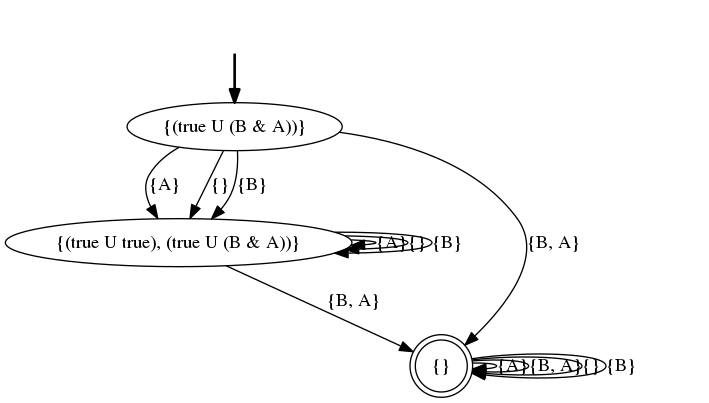
\includegraphics[width=\textwidth]{images/my_nfa}
		\caption{\texttt{nfa.to\_dot("my\_nfa")}}
		\label{fig:flloat-to_automaton-example-my-nfa}
	\end{subfigure}
	\begin{subfigure}[b]{0.40\textwidth}
		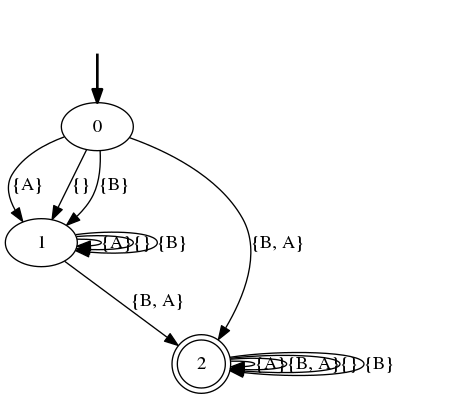
\includegraphics[width=\textwidth]{images/my_nice_nfa}
		\caption{\texttt{nfa.map\_to\_int().to\_dot("my\_nice\_nfa")}}
		\label{fig:flloat-to_automaton-example-my-nice-nfa}
	\end{subfigure}
	\caption{Examples of conversion from \LLf to \NFA and conversion into SVG images.}
\end{figure}

\subsection{On the fly evaluation of \LLf formulas}\label{sect:flloat-on-the-fly-evaluation}
FLLOAT supports also the on-the-fly evaluation of \LLf formulas, i.e. whether a finite trace satisfies an \LLf without building the entire automaton (see Section \ref{sect:on-the-fly-dfa}).

\begin{lstlisting}[language=Python, style=Python, escapechar = £, label={code:on-the-fly-dfa-example}, caption={From \LLf to \NFA}]
from flloat.parser.ltlf import LTLfParser
parser = LTLfParser()
formula = parser("F(A & B)")

dfaotf = formula.to_automaton(on_the_fly=True)£\label{code:on-the-fly-dfa-instruction}£

\end{lstlisting}

In Listing \ref{code:on-the-fly-dfa-example} it is shown how to use this feature. Notice that the method used, \texttt{to\_automaton}, is the same used in Section \ref{sect:flloat-llf2nfa} for the \LDLfToNFA algorithm, but with the flag \texttt{on\_the\_fly} set to \texttt{True}. In this case, \ref{code:on-the-fly-dfa-instruction} returns an object of the class \href{https://github.com/MarcoFavorito/flloat/blob/0.1.4/flloat/flloat.py#L164-L246}{flloat.flloat.DFAOTF}, that implements the concept explained in Section \ref{sect:on-the-fly-dfa}.

\begin{lstlisting}[language=Python, style=Python, escapechar = £, label={code:DFAOTF}, caption={The class \texttt{DFAOTF}, that implements on-the-fly \LLf formula evaluation.}]
class DFAOTF(Simulator):
"""DFA on the fly"""

  def __init__(self, f):
    self.f = f.to_nnf()
    self.reset()

  def reset(self):
    self.cur_state = frozenset([frozenset([self.f])])

  def word_acceptance(self, action_set_list:List[PLInterpretation]):
    self.reset()
    for a in action_set_list:
      self.make_transition(a)
    return self.is_true()

  def is_true(self):
    return self._is_true(self.cur_state)

  @staticmethod
  def _is_true(Q):
    ...

  def get_current_state(self):
    return self.cur_state

  def make_transition(self, i:PLInterpretation):
    self.cur_state = self._make_transition(self.cur_state, i)

  @staticmethod
  def _make_transition(Q, i: PLInterpretation):
    ...
\end{lstlisting}

In Listing \ref{code:DFAOTF} it is shown the implementation of the class \texttt{DFAOTF}, that you can find in the module  \href{https://github.com/MarcoFavorito/flloat/blob/0.1.4/flloat/flloat.py}{flloat/flloat.py}. It extends \texttt{Simulator}, which is a Pythomata abstract class for inherit \texttt{word\_acceptance} interface method. For the sake of brevity, we omitted some methods that have many lines. In the following we briefly describe the main methods:
\begin{itemize}
	\item \texttt{reset()} set the current state to the initial macro  state $\set{\set{\varphi}}$ notice that here (and in many other places) we used the data structure \texttt{frozenset}, which is an hashable set. This is useful for deal with \emph{sets of sets} (e.g. macro states);
	\item \texttt{\_\_init\_\_} is the constructor that takes in input a \LLf formula, compute its NNF and reset the state to the initial state \texttt{reset};
	\item \texttt{is\_true()}, whose implementation depends on \texttt{\_is\_true()} returns \texttt{True} if the current state contains the empty conjunction $\emptyset$, which stand for $\true$ (see Section \ref{sect:on-the-fly-dfa} for more details);
	\item \texttt{word\_acceptance} takes in input a finite trace (i.e. a list of propositional interpretations) and returns \texttt{True} if the last state contains the empty conjunction (see \texttt{\_is\_true()});
	\item \texttt{make\_transition} and \texttt{\_make\_transition} implements the computation of the next macro state, given a macro state and a propositional interpretation. In other words, they implements the progression rule for macro states, stated in Equation \ref{eq:on-the-fly-progression-rule}.
\end{itemize}

Typical uses of a \texttt{DFAOTF} instance are evaluation of finite traces. By continuing with Listing \ref{code:on-the-fly-dfa-example}, you can do it manually:

\begin{lstlisting}[language=Python, style=Python]
from flloat.semantics.pl import PLInterpretation
from flloat.semantics.pl import PLFalseInterpretation

A = PLInterpretation.fromStrings(["A"])
B = PLInterpretation.fromStrings(["B"])
empty = PLFalseInterpretation()
AB = PLInterpretation.fromStrings(["A", "B"])

dfaotf.make_transition(empty)
dfaotf.make_transition(A)
dfaotf.make_transition(B)
dfaotf.is_true() #False
dfaotf.make_transition(AB)
dfaotf.is_true() #True
\end{lstlisting}

Or by simply calling \texttt{word\_acceptance} over a list of \texttt{PLInterpretation}:
\begin{lstlisting}[language=Python, style=Python]
from flloat.semantics.ldlf import FiniteTrace

t1 = FiniteTrace.fromStringSets([
{},
{"A"},
{"B"},
{"A", "B"},
])

dfaotf.word_acceptance(t1.trace) #True
\end{lstlisting}

\subsection{From \LLf formula to \DFA}
Here we describe how FLLOAT supports the transformation from \LLf formulas to \DFA, i.e. the \LDLfToDFA algorithm (Algorithm \ref{alg:ldlf2dfa}). 

We adapt Listing \ref{code:llf2nfa} by simply using the same method \texttt{to\_automaton} but setting up the flag \texttt{determinze} to \texttt{True}.
\begin{lstlisting}[language=Python, style=Python, escapechar = £, label={code:llf2dfa-example}, caption={From \LLf to \DFA}]
from flloat.parser.ltlf import LTLfParser
parser = LTLfParser()
formula = parser("F(A & B)")

dfa = formula.to_automaton(determinize=True, minimize=False)£\label{code:llf2dfa-no-minimize-instruction}£

\end{lstlisting}

After the execution of these lines of code, in \texttt{dfa} is stored a \href{https://github.com/MarcoFavorito/pythomata/blob/master/pythomata/base/DFA.py}{\texttt{pythomata.base.DFA.DFA}} object that represents an equivalent \DFA. The method \texttt{LTLfFormula.to\_automaton} at line \ref{code:llf2dfa-no-minimize-instruction} dispatches the execution to the function \href{https://github.com/MarcoFavorito/flloat/blob/0.1.4/flloat/flloat.py#L48-L161}{\texttt{to\_automaton}} in \href{https://github.com/MarcoFavorito/flloat/blob/0.1.4/flloat/flloat.py#L249-L290}{flloat/flloat.py}, which implements \LDLfToDFA (Algorithm \ref{alg:ldl2nfa}). 

Now you can print the \DFA:
\begin{lstlisting}[language=Python, style=Python]
dfa.to_dot("my_dfa")
\end{lstlisting}

Quite often is better to obtain the minimized automaton:
\begin{lstlisting}[language=Python, style=Python]
dfa_min = formula.to_automaton(determinize=True, minimize=True)
dfa.to_dot("my_nice_dfa")
\end{lstlisting}
By simply calling the same method but with the flag \texttt{minimize} set to \texttt{True}.

Another equivalent approach is:
\begin{lstlisting}[language=Python, style=Python]
nfa = formula.to_automaton(determinize=False)
dfa = nfa.determinize()
dfa_min = dfa.minimize().trim()
dfa.to_dot("my_nice_dfa")
\end{lstlisting}


In Figure \ref{fig:flloat-to_automaton-example-my-dfa} and Figure \ref{fig:flloat-to_automaton-example-my-nice-dfa} are shown, respectively, the conversion to SVG images of the \DFA not minimized and the one minimized.
Notice how this representation is structurally identical to the one shown in \ref{fig:dfa-eventually-a}.
\begin{figure}[h]
	\centering
	\begin{subfigure}[b]{0.75\textwidth}
		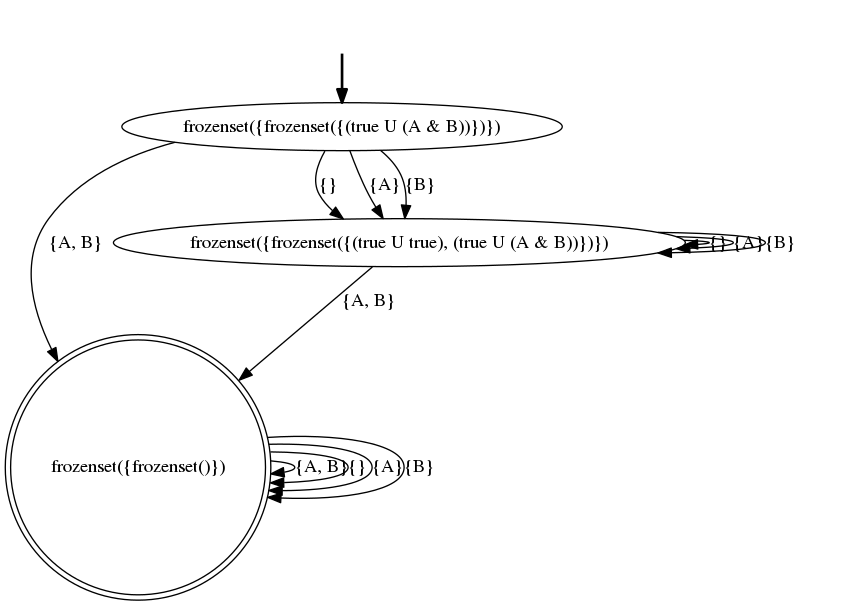
\includegraphics[width=\textwidth]{images/my_dfa}
		\caption{\texttt{dfa.to\_dot("my\_dfa")}}
		\label{fig:flloat-to_automaton-example-my-dfa}
	\end{subfigure}
	\begin{subfigure}[b]{0.40\textwidth}
		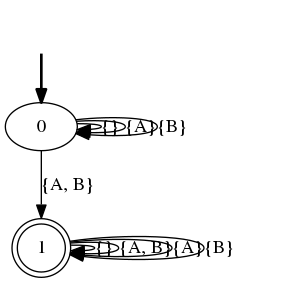
\includegraphics[width=\textwidth]{images/my_nice_dfa}
		\caption{\texttt{dfa\_min.to\_dot("my\_nice\_dfa")}}
		\label{fig:flloat-to_automaton-example-my-nice-dfa}
	\end{subfigure}
	\caption{Examples of conversion from \LLf to \DFA and conversion into SVG images.}
\end{figure}

\section{Conclusion}
In this chapter, we presented the FLLOAT Python package and its main features. We've seen the package structure, how FLLOAT supports \PL and \LLf formulas, and the conversion to automata from \LLf formulas.